\documentclass[10pt,conference,compsocconf]{IEEEtran}

%\usepackage{times}
%\usepackage{balance}
\usepackage{url, amsmath, amssymb}
\usepackage{graphicx}    % For figure environment
\usepackage{textcomp}
\usepackage{amsfonts}
\usepackage[ruled,vlined]{algorithm2e}

\usepackage[hidelinks,bookmarksnumbered,unicode]{hyperref} % Enables cross linking in the electronic document version. This package has to be included second to last.
\usepackage[noabbrev,nameinlink]{cleveref}
\usepackage{balance}
\usepackage{nag}       % Issues warnings when best practices in writing LaTeX documents are violated.
\usepackage{booktabs}
\usepackage{amsmath}   % Improves the typesettings of tables.

%\DeclareMathOperator*{\argmin}{\arg\!\min}
\DeclareMathOperator*{\argmin}{argmin}   % Jan Hlavacek

\newcommand{\spacing}{\hspace{1cm}}

\usepackage{xcolor}
\newcommand{\todo}[1]{\textcolor{red}{#1}}
%\newcommand{\todo}[1]{{\color{red}{#1}}}

\begin{document}
    \title{On Bayesian Factorization Machines in Collaborative Filtering}

    \author{
        Rafael Sterzinger \spacing Patrik Okanovic \spacing Fatjon Zogaj \spacing Filip Batur Stipic\\
        Group: Terminators\\
        Department of Computer Science, ETH Zurich, Switzerland
    }

    \maketitle

    \begin{abstract}
        Collaborative Filtering offers promising results for the task of Recommender Systems.
        In this work we compare several neural-based and standard matrix factorization methods, placing our focus on Bayesian Factorization Machines.
        We build upon Bayesian Factorization Machines by including implicit user/item information, distance similarities and genre clustering and report results in an extensive benchmark.

    \end{abstract}


    \section{Introduction}

    The goal of recommender systems is to design a model which is capable of estimating a user's preference on some kind of items, in our case movies.
    This is usually done by means of collaborative filtering, a standard computational method that attempts to solve this problem by leveraging similarities between users and items based on previously collected data in some vector space~\cite{CF_survey}.
    This data usually consists of user/item pairs and its corresponding rating which is normally presented in form of a real-valued sparse matrix.
    This sparseness stems from the majority of user/item pairs being unavailable.

    In this project we are concerned with completing such a sparse matrix in the setting of movie recommendation systems, a problem for which benchmarks such as the Netflix Prize~\cite{Netflix} and the different versions of MovieLens~\cite{Movielens} are already well-established.
    As such, we viewed these benchmarks as guidelines to select 7 state-of-the-art models allowing for a rigorous evaluation of our final results.

    Among these baselines, we selected standard techniques, mainly based on matrix factorization.
    These include Singular Value Decomposition~\cite{svd}, Non-Negative Matrix Factorization~\cite{6165290}, and different variants Bayesian Factorization Machines~\cite{freudenthaler_bayesian_2011, salakhutdinov_bayesian_2008}.

    As an alternative, we explored different, more recent neural network based methods such as Neural Collaborative Filtering~\cite{DBLP:journals/corr/abs-1708-05031}, autoencoders~\cite{inproceedings} and other autoencoder-like networks.
    Here, we selected the Kernel Net~\cite{pmlr-v80-muller18a}, and the AutoRec model~\cite{inproceedings}.


    \section{Models and Methods}
    In the following section we provide a brief overview of our different baselines, which served as a starting point for exploring the field of collaborative filtering.

    \subsubsection{Preprocessing: Missing Values Initialization}\label{subsub:missing_init}
    As the majority of our models depends on the whole data matrix as input, we experiment with a variety of initialization techniques for the unobserved/missing values.
    Our approaches include replacement by the total mean, user mean and item mean of rankings.
    We add upon this by enabling a model to be used for predicting the missing values that then get used as input for another model.
    This also allows us to iteratively chain multiple models to predict the unobserved values for the respective following one.

    \subsubsection{Postprocessing: Clipping/Rounding}
    As a final step after the prediction we try various ways of postprocessing the output.
    The default way is a simple clipping between 1 and 5.
    As the rankings are given as integers, values such as 1.15 do not make a lot of sense.
    A prediction of the model to be closer to 1 than 2, leads to an "unnecessary" error when it guesses correctly, but outputs real values.
    We try rounding the outputs to the nearest integer as well as to the nearest quarter.

    \subsection{Standard Matrix Factorization based Approaches}

    \subsubsection{Singular Value Decomposition (SVD)}

    SVD is a matrix factorization technique that decomposes the original matrix $A \in {\rm I\!R}^{m*n} $ into the form $ A = U \Sigma V $ where $U \in {\rm I\!R}^{m*m}$,  $V  \in {\rm I\!R}^{m*n}$ are orthogonal matrices and $\Sigma \in {\rm I\!R}^{m*n}$ is a diagonal matrix whose entries are called singular values.

    To apply SVD for Collaborative filtering we assume there exists a latent feature vector for each individual user and movie, so that the rating can be determined by taking the inner product between the feature vectors for the corresponding user and movie.
    Since the matrix is sparse, we initialize the missing values as mentioned in \Cref{subsub:missing_init}, and apply SVD to obtain the latent feature vectors from the columns of the matrices $U$ and $V$~\cite{svd}.

    Since low-rank approximations can be more generalizable, we usually only keep the $k$ best feature vectors for both users and movies associated with the $k$ largest singular values~\cite{Eckart1936}.%, which is guaranteed to give the best approximation out of all k-rank matrices~\cite{Eckart1936}.

    One downside of SVDs lies in being highly sensitive to the initialization of the imputed missing values, whereas the benefits are that SVDs always exist, are easy to compute and are readily available in standard libraries.

    \subsubsection{Non-Negative Matrix Factorization (NMF)}

    Since the ratings in the matrix are non-negative, another feasible approach is to consider Non-Negative Matrix Factorization, which decomposes our original matrix into $A = WH$, where $W$ and $H$ are both non-negative~\cite{gillis2014nonnegative}.
    Commonly, it achieves this by optimizing over the Frobenius norm between the difference of the observed entries of the approximation and the original matrix:

    $$ \frac{1}{2}\|\Pi_{\Omega}(A - WH)\|^2_F$$

    Although this optimization problem is NP-hard, in practice we can obtain good solutions by leveraging the separability of parameters that depend on U and V respectively, for example by using the Alternating Least Squares algorithm~\cite{als}.

    \subsubsection{Bayesian Factorization Machines (BFM)}
    For our last standard matrix factorization based approach, we explored Bayesian Factorization Machines BFM which are Bayesian variants of the former known Factorization Machines (FM)~\cite{rendle_factorization_2010}.
    In its core, FMs build upon the advantages of Support Vector Machines (SVM) but use a factorized parametrization instead of a dense one.
    With this parametrization, FMs are able to estimate all possible interactions between entries of $\mathbf{X}$ even in setting where the data matrix $\mathbf{X}$ is highly sparse.
    Similarly to SVMs with a polynomial kernel, the FM model equation which captures all single and pairwise interactions, can be formulated as follows:

    $$\hat{y}(\mathbf{x})=w_0+\sum^n_{i=1}w_ix_i + \sum^n_{i=1}\sum^n_{j=i+1}\langle \mathbf{v_i},\mathbf{v_j} \rangle x_ix_j$$

    Here, $v_i$ denotes a vector in $\mathbb{R}^k$ which describes the $i$-th variable with $k$ dimensions and $\langle \mathbf{v_i},\mathbf{v_j} \rangle$ the interaction between the variables $i$ and $j$.
    Instead of using a fixed weight $w_{ij}$, this factorization via the dot product allows FMs to predict parameters for related interaction, e.g. different users but same movie.
    In the non-Bayesian setting, model parameters are optimized with stochastic gradient descent.
    As opposed to this, model parameters of Bayesian variants of FMs are optimized via maximum a posteriori estimation by means of Markov Chain Monte Carlo methods for approximate inference~\cite{salakhutdinov_bayesian_2008}.
    This Bayesian approach does not only increase accuracy but also omits the need of exhaustive parameter tuning~\cite{freudenthaler_bayesian_2011}.
    Regarding the implementation of our baseline, we utilize a package named \textit{myFM}~\cite{noauthor_myfm_nodate} which employs Gibbs sampling for approximate inference of the posterior.
    Multiple additions have been made by means of exploiting additional implicit information about users, items, and temporal dynamics~\cite{rendle_scaling_2013,koren_factorization_2008,koren_collaborative_2009}.
%    We incorporate the majority of these, omitting temporal dynamics due to the absence of this information in our provided dataset.
%    In our implementation, we incorporated most of these as well, omitting temporal dynamics due to the absence of this information in our provided dataset.
    The two implicit features we add are defined as follows:
    \begin{enumerate}
        \item Implicit User Feature (Bayesian SVD++) $\Leftrightarrow$ all items rated by user $u$:
        $$\mathbf{V}_u=\frac{\Omega_u}{\sqrt{|\{(u,i): (u,i) \in \Omega_u\}|}}$$
        \item Implicit Item Feature (Bayesian SVD++ flipped) $\Leftrightarrow$ all users that rated item $i$:
        $$\mathbf{W}_i=\frac{\Omega^T_i}{\sqrt{|\{(u,i): (u,i) \in \Omega^T_i\}|}}$$
    \end{enumerate}
    After one-hot-encoding users $\mathbf{U}$ and items $\mathbf{I}$, denoted as the identity matrix $I_k$ with corresponding dimension $k$, a single entry in our dataset has the following form:
    $$\mathbf{x}_{ui} = [(I_n)_u,\mathbf{V}_u,(I_m)_i,\mathbf{W}_i, r_{ui}]$$

    Additionally, datasets commonly used in the setting of collaborative filtering such as the MovieLens dataset include much more detailed information on users/items.
    In the setting of movie recommendations, for instance, the genre or the release date of a movie, a timestamp of when the user gave the rating, or user specific information such as who is friends with whom might be included.
    These details contain valuable information and as such, we try to recreate features resembling those. % ones based on the limited data we were provided.
    Here, we concentrated mainly on two aspects, calculating the similarity between users to imitate the "friends of a user" feature, and clustering a movie embedding space to create a "movie genre" feature.

    \paragraph{User Features}
    To embed similarity measures between two users, we analyzed variants of the Jaccard index, the standard one and an improved version of it~\cite{lee_improving_2017}.
    The standard Jaccard index measures the similarity between two users $u$ and $v$ as follows:
    $$\text{Jac}(u,v)=\frac{|\mathbf{I}_u \cap \mathbf{I}_v|}{|\mathbf{I}_u \cup \mathbf{I}_v|}$$
    Furthermore, we experimented with an improved version of the Jaccard index.
    Here, the set of items $\mathbf{I}_u$ a user $u$ has rated is subdivided into three parts $L,M,$ and $H$ with two boundaries $L_{bd}$ and $H_{bd}$.
    Given these boundaries the sets are formulated as follows:
    \begin{align*}
        &\mathbf{I}_{L,u}=\{i \in \mathbf{I}_u : r_{u,i} \leq L_{bd}\}\\
        &\mathbf{I}_{M,u}=\{i \in \mathbf{I}_u : L_{bd} < r_{u,i} < H_{bd}\}\\
        &\mathbf{I}_{H,u}=\{i \in \mathbf{I}_u : H_{bd} \leq r_{u,i}\}\\
    \end{align*}
    The improved Jaccard index with these definied subsets is denoted as follows:
    $$\text{Jac}_{LMH}=\frac{1}{3}(\text{Jac}_L(u,v) + \text{Jac}_M(u,v) + \text{Jac}_H(u,v))$$
    According to the authors the bound $L_{bd} = 3$ and $H_{bd}=4$ yielded the best results on the MovieLens dataset.
    As such, we set the same bounds, effectively splitting into two instead of three sets.

    \paragraph{ Movie Features}
    To imitate movie categories as in the MovieLens dataset we implement a clustering mechanism.
%    In order to provide additional information for models, we implement clustering and that way provide the information about movie categories as in the MovieLens dataset.
    First we initialize the matrix using BFM.
    Afterwards, we perform Singular Value Decomposition with rank 10 (best result of \Cref{fig:rank}).
    We get the embeddings using the following expression: assuming $A=U\Sigma V^T$ then the matrix corresponding to the movie embeddings is equal to $\Sigma _k ^{\frac{1}{2}} V_k ^T$.
    Finally, after obtaining the rank $k$ movie embeddings, we search for the optimal number of clusters in K-Means clustering.
    Since, visualizing in two dimensions does not easily distinct the optimal number of clusters we choose 18 as in the MovieLens dataset as the number of clusters/genres.

    The following \Cref{alg:algo1} shows our proposed procedure for creating additional features to run \textbf{BFM}

    \begin{algorithm}
        \SetKwInOut{Input}{input}
        Initialize missing matrix value with FM\\
        $k_{opt}=\argmin_{k}$ RMSE(SVD$_{rank=k}(\mathbf{ X })$\\
        $\mathbf{E} = \sqrt{\Sigma_{k_{opt}}}V_{k_{opt}}^T$ \# Embedding\\
        $\mathbf{ G }$ = K-Means($e$) \# Clustering\\
        \For{$i = 0...m$} {
            \For{$j = 0...m$} {
                $D_{i,j} ^{Eucl} = \|E_i - E_j\|_2$ \\
                $D_{i,j} ^{Mahal} = \sqrt{(E_i-E_j)^TCov^{-1}(E_i-E_j)}$
            }
        }
        \Return{$G, D^{Mahal},D^{Eucl}$}
        \caption{Novel Feature Creation}
        \label{alg:algo1}
    \end{algorithm}

    With these additional user/item features, we append to our feature vector $\mathbf{x}_{ui}$ a dense vector of user similarities from user $u$ to every other user, or the item feature which is either the one-hot-encoded cluster of item $i$ or a dense vector of Euclidean/Mahalanobis distances from item $i$ to every other item.

    Finally, for our best model, we reformulate the task of predicting unobserved user/item pairs to a classification problem instead of a regression task where we calculate the expectation over the different class probabilities.

    \subsection{Neural Network based Approaches}

    \subsubsection{Neural Collaborative Filtering (NCF)}
    Neural Collaborative Filtering as proposed by He et al.~\cite{DBLP:journals/corr/abs-1708-05031}
    jointly learns user-item latent representations and predictions based on the interactions between
    different users and items.
%    The network's inputs are indices of users and items.
    An embedding layer maps each user and each item to its corresponding latent vector representation.
    These outputs are then concatenated and passed on through fully connected feedforward layers with ReLU activation functions to form the predictions.
    We train the model by minimizing the mean squared error loss.
%    Finally, output of the network represents the rating associated with the inputted user and item.
%    We use the mean squared error loss between the output of  and target rating.
%    Network is trained minimizing the mean squared error loss between the predicted and target rating.

    \subsubsection{Autoencoder (AE)}
    An AE is a neural network consisting of an encoder $f: \mathbb{R} ^d \rightarrow \mathbb{R} ^k$ and a
    decoder that produces a reconstruction $g: \mathbb{R} ^k \rightarrow \mathbb{R} ^d$~\cite{Goodfellow-et-al-2016}.
    It is trained to recreate its input as its output $\mathbf{ \hat{x} } = g(f(\mathbf{x}))$.
    Autoencoders have proven to achieve good results in collaborative filtering~\cite{inproceedings}.
    We examine the user-based AE as opposed to item-based AE which achieved a good score in~\cite{inproceedings}.
    Both encoder and decoder consist of feedforward neural networks with ReLU activation functions.
    We train the model by minimizing the squared reconstruction loss.
%    Important part of the implementation is the fact that inputs are partially observed and therefore we only update those weights that are associated with observed inputs during backpropagation.

    \subsubsection{AutoRec}
    Based on the previous model, we have added the AutoRec implementation~\cite{inproceedings}, which achieved a state-of-the-art result.
    Compared to our AE implementation AutoRec is item-based, uses the sigmoid activation function as the final non-linearity and adds regularization to the loss function.

    \subsubsection{Kernel Net}
    We add the MovieLens-1M state of the art model (on papers with code\todo{add cite for this }),
    for which we adapt the code from~\cite{pmlr-v80-muller18a, kernelNetGithub} into our experiment framework.
%    as another baseline as the given problem description fares very similarly to ours.
%    For this, we adapt the code from~\cite{pmlr-v80-muller18a, kernelNetGithub} into our experiment framework.

%    The high sparsity in recommender-system datasets leads to the need and resulting variety of possibilities for dimensionality reduction.
%    Combined with the amount of parameters in neural networks this leads to large training times and possibly
%    unexpected results on unseen data due to overfitting.

    Muller et al. make use of finite-support kernels to reparametrize weight matrices with low-dimensional vectors.
    This allows for the structured feature embedding of neural network weights based on the specific kernel function used and
    acts as regularization.
    As such, their item-based AE is able to reduce complexity at inference time while improving performance compared to similar models\cite{pmlr-v80-muller18a}.


    \section{Results}
    We present our results in \Cref{tab:ablation}, noting the Root Mean Squared Error (RMSE) of our baselines and final model.
    Test scores refer to the public leaderboard ranking on Kaggle while validation scores refer to a 10\% holdout of our training data.
    \todo{isn't this clear}Here, it is important to note that test scores reported for standard matrix factorization models where obtained by training on the whole data.
    Models without test scores are added for the sake of completeness and not evaluated further as the performance was either not satisfactory or other models evaluated in the meantime performed better.
    Other models may only show test scores as they were directly evaluated on the test data to eliminate the need of
    fitting a second time.

    All scores are reported after clipping the outputs to a range between 1 and 5 unless stated otherwise.% or, if stated otherwise, rounded to the closest quarter.

    Our first baseline, SVD with rank 3, heavily depends on the initialization of unobserved values, achieving a test score of 0.9928 when replacing values with the item mean and only 1.0713 when using the overall mean.
%    This illustrates that using the item mean over other variants seems superior and based on this,
    Due to this large discrepancy, we further experimented with more sophisticated initialization techniques such as using other models to predict unobserved values.
    In \Cref{tab:ablation}, \textit{10*SVD} stands for chaining SVD ten times one after another to iteratively predict unobserved values (leaving the observed values as is) for the input of the following.
%    where after each round we reset the observed entries back to their original values.
    With this we were able to get a test score of 0.9882 which is a large improvement for SVD.
    Similar to this, \textit{SVD + KernelNet} first trains the KernelNet and then predicts the unobserved values such that they can be used to initialize the SVD.
    This further decreased the error to 0.9836 which is the best test score we achieved using SVD.
%    An additional experiment that we conducted, was the idea to initialize SVD with the output of a BFM SVD++ flipped predictor and perform SVD iteratively multiple times.
    Using our best final BFM model chained with \textit{5*SVD} we achieve a test error of 0.9846.
    \todo{Rafi results, change above Kernel Sentence if better than that}

%    While this approach unsurprisingly performs well in regards to the better initialization of unobserved values in SVD, it did not improve upon the BFM variant.


    Similar to the SVD, our second baseline, NMF, performs best when replacing missing values with the item mean and then chaining 10 NMF models which results in a validation score of 0.9946.

    We varied the amount of singular values to keep and reported the average performance of 3-fold cross validation.
    Looking at \Cref{fig:rank}, we see that except for NMF, which achieves the lowest error with rank 24, the other standard matrix factorization models perform best with a lower rank approximation of around 10.
    \begin{figure}
        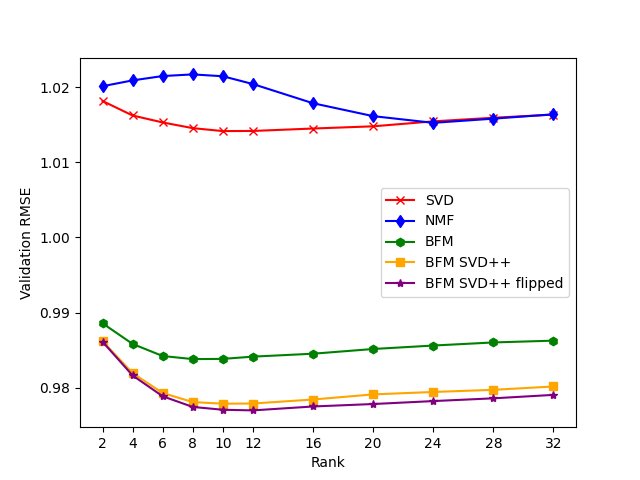
\includegraphics[width=\columnwidth]{figures/rank.png}
        \caption{Validation RMSE for different rank values when trained on a 90/10 train/test split.
        NMF performs best with a rank of 24 while others peak around 8 to 12.}
        \label{fig:rank}
    \end{figure}

    Next, we evaluate neural network based approaches.
    Starting with standard AE, we found that, when both the encoder and the decoder consist of a single hidden layer, increasing the width resulted in a better score.
    Furthermore, we have examined the effect of compositionality by using two layers which outperformed any single layer network, obtaining a validation score of 1.0539 after 250 epochs.
    \todo{Patrik Check epochs of table and figure as well as result.}
    NCF, our fourth baseline, already surpasses this performance only after 10 epochs and achieves its best score of 0.9787 after epoch 250.
    Compared to that is the AutoRec which achieved an RMSE of 1.0100 after only 5 epochs after which the error steadily increased.
    Regarding the KernelNet, replacing the unobserved values with zeros instead of item mean surprisingly fared best which is in contradiction to the insights gained from SVD, leading to a much better validation error of 0.9831 as opposed to 1.0409 (both 150 iterations).

    From \Cref{fig:validation} it can be observed that overall the KernelNet performed best, the AE made continuous progress, while AutoRec and NCF quickly started to overfit and diverge.

    \begin{figure}
        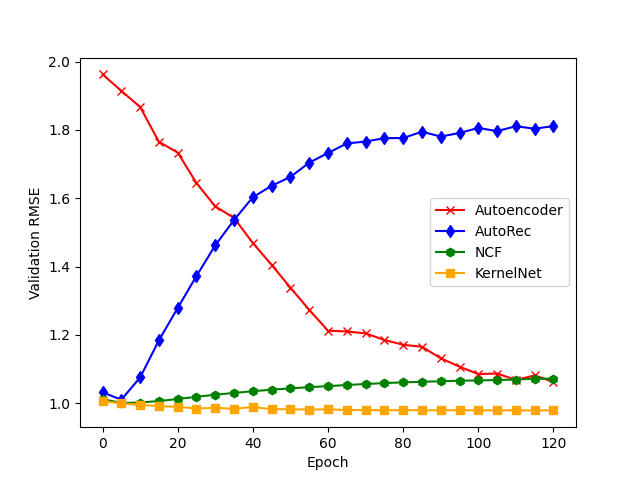
\includegraphics[width=\columnwidth]{figures/validation_plot.png}
        \caption{Validation RMSE for different epochs when trained on a 90/10 train/test split.
        AutoRec and NCF started to diverge after a few epochs while KernelNet and Autoencoder show the opposite behaviour.}
        \label{fig:validation}
    \end{figure}

    Regarding our final baseline, the standard BFM, we obtained similar results to~\cite{rendle_difficulty_2019}.
%    \todo{refer to respective table or appendix}
    As can be seen in \Cref{tab:ablation}, including both implicit user and movie features to BMF improves the score.% than standard BFM and BFM with only implicit user features.
    Adding additional features for users and movies resulted in similar performance compared to the BFM SVD++ flipped model
    for almost all of our proposed features.
    However, we noticed that including the distance metrics performed worse when compared to the genre clustering.%, hinting that with some fine-tuning of the cluster sizes, better results might be achievable.

    Genre clustering with size 18 performed very similar to the BFM SVD++ flipped, which might suggest that with some hypertuning improvements are possible.
    We leave this off to future work due to limited resources as one evaluation takes on the order of days.

    Compared to that, the introduction of the Jaccard index% to resemble connections between users
    performed similarly as well whereas the improved version of it surprisingly decreased the performance.
    As a final approach, we reformulated the problem of predicting user/movie ratings from a regression problem into a classification one which yielded a slight performance gain (Ordered Probit).

%    A general overview of low rank matrix approximation techniques can be observed in \Cref{fig:rank}.
%    Here, we varied the amount of singular values to keep and reported the average performance of 3-fold cross validation.
    The heatmap, illustrated in \Cref{fig:Heatmap}, gives an overview on the conducted parameter search of sampling size per iteration and ranks for the BFM SVD++ flipped.

    \begin{table}
        \centering
        \resizebox{\columnwidth}{!}{
            \begin{tabular}{|| c | c | c | c | c ||}
                \hline
                \textbf{Model}       & \textbf{Params}                       & \textbf{ Init Missing } & \textbf{RMSE}$_{test}$ & \textbf{RMSE}$_{valid}$ \\
                \hline
                SVD                  & Rank 3                                & total mean              & 1.0713                 &                         \\
                SVD                  & Rank 3                                & user mean               & 1.0558                 &                         \\
                SVD                  & Rank 3                                & item mean               & 1.0138                 &                         \\
                4*SVD                & Rank 3                                & item mean               & 0.9928                 & 0.9893                  \\
                7*SVD                & Rank 3                                & item mean               & 0.9894                 &                         \\
                10*SVD               & Rank 3                                & item mean               & 0.9882                 & 0.9854                  \\
                10*SVD               & Rank 3, Round Quarters                & item mean               & 0.9907                 &                         \\
                10*SVD               & Rank 10                               & item mean               & 0.9941                 &                         \\
                5*SVD + KernelNet    & Rank 3 | 150 Epochs                   & zero                    &                        & 0.9844                  \\
                5*SVD + KernelNet    & Rank 10 | 150 Epochs                  & zero                    &                        & 0.9838                  \\
                SVD + KernelNet      & Rank 10 | 150 Epochs                  & zero                    & 0.9836                 & 0.9803                  \\
                5*SVD + BFM SVD++ f. & Rank 3 | Rank 12                      & /                       & 0.9846                 &                         \\
                \hline
                NMF                  & Rank 24                               & total mean              &                        & 1.0628                  \\
                NMF                  & Rank 24                               & user mean               &                        & 1.0497                  \\
                NMF                  & Rank 24                               & item mean               &                        & 1.0029                  \\
                10*NMF               & Rank 24                               & item mean               &                        & 0.9946                  \\
                \hline
                AE                   & 50 Epochs                             & total mean              &                        & 1.3382                  \\
                AE                   & 150 Epochs                            & total mean              &                        & 1.0757                  \\
                AE                   & 250 Epochs                            & total mean              &                        & 1.0539                  \\
                \hline
                NCF                  & 50 Epochs                             & /                       &                        & 1.0394                  \\
                NCF                  & 150 Epochs                            & /                       &                        & 1.0756                  \\
                NCF                  & 250 Epochs                            & /                       &                        & 1.0845                  \\
                \hline
                AutoRec              & 5 Epochs                              & zero                    &                        & 1.0100                  \\
                AutoRec              & 25 Epochs                             & zero                    &                        & 1.3723                  \\
                AutoRec              & 50 Epochs                             & zero                    &                        & 1.6625                  \\
                \hline
                KernelNet            & 50 Epochs                             & zero                    & 1.0003                 & 0.9939                  \\
                KernelNet            & 150 Epochs                            & zero                    & 0.9860                 & 0.9831                  \\
                KernelNet            & 150 Epochs                            & item mean               &                        & 1.0409                  \\
                KernelNet            & 450 Epochs                            & zero                    & 0.9886                 &                         \\
                \hline
                BFM                  & Rank 12                               & /                       &                        & 0.9727                  \\
                BFM SVD++            & Rank 12                               & /                       &                        & 0.9664                  \\
                BFM SVD++ f.         & Rank 12                               & /                       & 0.9688                 & 0.9655                  \\
                BFM SVD++ f.         & Jac. Sim., Rank 32                    & /                       & 0.9694                 &                         \\
                BFM SVD++ f.         & Improved Jacc. Sim., Rank 32          & /                       & 0.9974                 &                         \\
                BFM SVD++ f.         & Genre Clustering, Rank 32             & /                       & 0.9688                 &                         \\
                BFM SVD++ f.         & Mahalanobis Dist., Rank 32            & /                       & 1.0271                 &                         \\
                BFM SVD++ f.         & Euclidean Dist., Rank 32              & /                       & 0.9903                 &                         \\
                BFM SVD++ f.         & Ordered Prob., Rank 32                & /                       & \textbf{ 0.9657 }      &                         \\
                BFM SVD++ f.         & Ordered Prob., Round Quarter, Rank 32 & /                       & 0.9684                 &                         \\
                \hline
            \end{tabular}
        }
        \caption{We note the Root Mean Squared Error (RMSE) on test and validation datasets to compare our baselines to our novelties.}
        \label{tab:ablation}
    \end{table}


    \begin{figure}
        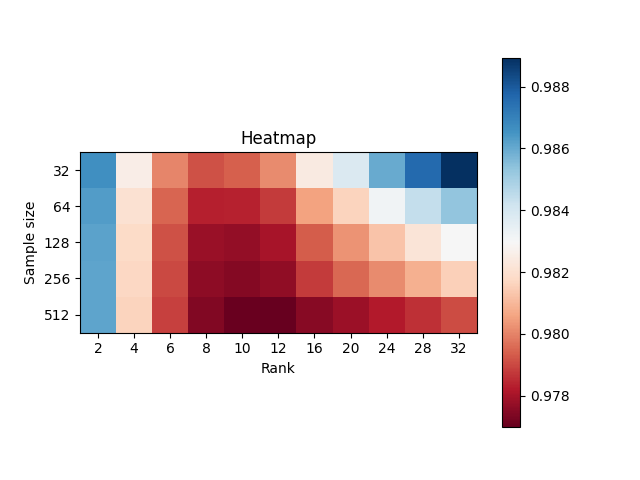
\includegraphics[width=\columnwidth]{figures/heatmap.png}
        \caption{Validation RMSE for different values of sample size and rank when trained on a 90/10 train/test split. Note that this parameter search has been conducted on our second best model, BMF SVD++ flipped, due to the high computational burden of our best model.
        A low-rank approximation of 8 to 12 with the highest sampling size performs best.}
        \label{fig:Heatmap}
    \end{figure}


    \section{Discussion}
    As stated in the previous section, the introduction of additional hand-crafted features for users and movies did not yield significant improvements.
    We assume that this is mainly based on the statistical learning theory fact that one cannot gain additional information out of existing data.
    Although, the genre clustering as well as the standard Jaccard index did not perform much worse than the standard baselines, we conclude that hand-crafting features for collaborative filtering is not a direction worth exploring.

    However, using more sophisticated postprocessing techniques like rounding to integers or to quarters always resulted in worse performance.
    % TODO primarily BMF

    This might be due to the fact users tend to overall rate movies rather positive than negative for which we assume that this phenomenon can be better captured by formulating the problem of predicting user/movie ratings as a classification task.
    %TODO importance of shuffeling
    %add info that we trained on whole dataset


    higher sampling size is better, rank of 12 seems to be optimal but not for classification.


    \section{Summary}

    In this paper we have examined the problem of collaborative filtering, analyzing a variety of models, such as SVD, NMF, NCF, KernelNet, and AE networks.
    We explore variants of Bayesian Factorization Machines, improving upon the score of the selected baselines.
    We extend BFMs with additional features that represent movie genre, similarities between movies/users and implicit friend of a user information making it more accessible and explicit.



    \balance
    \bibliographystyle{IEEEtran}
    \bibliography{bibliography}
\end{document}
